\documentclass[12pt]{article}
\usepackage{amsmath,amsfonts,amsthm,amssymb,wasysym}
\usepackage{setspace}
\usepackage{enumitem}
\usepackage{Tabbing}
\usepackage{fancyhdr}
\usepackage{lastpage}
\usepackage{chngpage}
\usepackage{url}
\usepackage{subfigure}
\usepackage{array}
\usepackage{multicol}
\usepackage[color=blue!40]{todonotes}
\usepackage[protrusion=true,expansion,kerning]{microtype}
\usepackage{natbib}

% to adjust margins:
\topmargin=-0.25in
\evensidemargin=0in
\oddsidemargin=0in
\textwidth=6.25in
\textheight=8.5in
\headsep=0.25in

% homework specific information
\newcommand{\hmwkTitle}{CS689 Final Project}
\newcommand{\hmwkDueDate}{December 6, 2013}
\newcommand{\hmwkClass}{}
\newcommand{\hmwkClassInstructor}{}
\newcommand{\hmwkAuthorName}{Patrick Verga \\ Emma Strubell}

% header and footer
\pagestyle{fancy}
\lhead{\hmwkAuthorName}
\chead{\hmwkTitle}
\rhead{\hmwkDueDate}   
\lfoot{}
\cfoot{}
\rfoot{\emph{Page\ \thepage\ of\ \pageref{LastPage}}}                          
\renewcommand\headrulewidth{0.4pt}
\renewcommand\footrulewidth{0.4pt}

\makeatletter
\newenvironment{tablehere}
  {\def\@captype{table}}
  {}

\newenvironment{figurehere}
  {\def\@captype{figure}}
  {}
\makeatother

%\renewcommand{\bibsection}{\subsubsection*{\refname}}

% Make title 
\title{
\LARGE\bf Author Attribution of Yelp Reviews \\
\date{}
\author{ Emma Strubell \and Patrick Verga}
}

\begin{document}

\maketitle

\begin{abstract}
We attempt to identify the authors of Yelp reviews using two versions of $k$-means clustering and support vector machines.
\end{abstract}

\thispagestyle{fancy}

%\begin{multicols}{2}

\section{Introduction}
Author attribution, the ability to identify the author of a given document given its text, has implications for companies trying to identify fraud, law enforcement identifying posts by criminals or terrorists, and even historians working to discern the true creator of a disputed piece of text. These principles are similarly important for individuals seeking privacy or anonymity, such as dissidents of a repressive government. 

Companies such as Yelp, TripAdvisor, and Amazon who provide product or business reviews as a service to their customers rely on having accurate and truthful reviews of those products and businesses. However, companies or individuals may artificially inflate their own review score or deflate those of their competition. The ability to accurately and effectively identify and remove fraudulent reviews would be extremely beneficial to these companies to ensure the integrity of their product. In our work we attempt to apply principles of stylometry and author identification to the problem of fraud detection. 

\section{Background}
Stylometry is the analysis of individuals’ usage of linguistic features to attempt to identify those individuals. In some cases this can include standard information retrieval techniques such as term frequency-inverse document frequency  (TF-IDF) bag-of-words approaches. However, using bag-of-words has the downside of capturing context specific variability rather than writing style variability. That is, differences in what the piece is written about rather than the way the piece is written.

There are several different ways to approach the problem of author identification. They can be broadly separated into two groups: classification and similarity detection. The more widely studied problem is that of classification. Given a set of authors each with a set of documents, one can train a model to then attribute a new unknown document to one of the known authors. The less-investigated problem is that of similarity detection. Here, instead of using a training corpus to define a small number of authors, one can use a technique such as clustering to partition a set of documents into different clusters that should correspond to different authors.

There is a great deal of existing research in the field of stylometry, some even predating computers; one of the earliest applications was attempting to discern the true author of the Federalists papers. More recently, researchers have attempted to classify authors of twitter posts \cite{Castro2012,Layton2010} and web forum posts \cite{Pillay2010,Tan2010}. \cite{Savoy2013} attempted to use topic modeling for author attribution.

Most attempts to discern authorship are performed on a very small set of authors each given a large corpora of training data. Some work has been done on internet scale problems given thousands or an unknown number of authors. \cite{Narayanan2012} attempted to classify posts of several thousand authors with moderate success. Their work was based off of the Writeprints model \cite{Abbasi2008} whose feature choices have become very influential. We crafted our feature set based on \cite{Narayanan2012}.

\section{Dataset}
Yelp's Academic Dataset\footnote{\protect\url{https://www.yelp.com/academic_dataset}} provides data and reviews for the 250 closest businesses to 30 universities in North America. We used the subset of the data for the city of Pheonix, Arizona. The data consists of three different types of JSON object: user objects, business objects, and review objects. For our task we were interested in the \texttt{user\_id} and \texttt{text} properties of the review objects, as well as the \texttt{review\_count} property of the user obejcts for further pruning of the data. In our actual experiments, we used the reviews of the 23 users who had written more than 250 reviews in an attempt to provide our learning algorithms with enough data to correctly classify the documents. Although the Yelp dataset provides additional information about the users and reviews that might be useful in user review classification, such as user star ratings and the date the review was posted, we elected not to use this data as features in order to avoid tuning our approach too exclusively to the review domain. Instead, we limited our features to those based on the review text only, and thus that could be applied to achieve author attribution on text from any domain, such as forum posts, blogs or emails.

\section{Methods}

\subsection{Features}
As noted in the previous section, we limited our features to those based on the text of the review. Based on \cite{Narayanan2012}, the features we used are listed in Table 1. 

\begin{figure}[h!]
\begin{center}
\begin{tabular}{ll}
\hline
{\bf Feature Type} & {\bf Description} \\ \hline
Document length & Number of words, characters in post \\
Vocabulary richness & Yule's $k$ \\
Word shape & Frequency of capitalization types (all, none, first, camel)\\
Word length & Frequency of words containing 1--20 letters\\
Letters & Frequency of letters a--z (case insensitive) \\
Digits & Frequency of digits 1--9 \\
Punctuation & Frequency of \texttt{.,!?;:()"'} \\
Special characters & Frequency of \url{~`@%#$%^&*_+=\{\}[]\\|/<>} \\
Function words & Frequency of function words; See text \\
Part-of-speech & Frequency of 50 different part-of-speech tags \\
Syntactic dependency label & Frequency of 50 different syntactic dependency labels
\end{tabular}
\caption{Table of features used in our model.}
\end{center}
\end{figure}

Syntactic features such as part-of-speech tags and dependency labels were generated using the natural language processing pipline included in FACTORIE \cite{mccallum09:factorie:}. In our computation of Yule's $k$ measure for vocabulary richness, we used standard WordNet \cite{wordnet} lemmas. We used the following equation to compute Yule's $k$:
\begin{align}
k &= 10000\frac{m_2-m_1}{{m_1}^2}
\end{align}

where $m_1$ is the number of distinct lemmas found in the document, and $m_2$ is defined in terms of $f_i$, the frequency of lemma $i$ in the document, and $c_i$, the count of lemma $i$ in the document:
\begin{align}
m_2 &= \sum_{i=1}c_if_i^2
\end{align}

In initial clustering experiments using bag-of-words features, we found that including frequencies of all words found in the text as features caused the algorithms to group reviews based on topic rather than author. This makes sense since the occurence of the word ``spicy'' in restaurant reviews is more likely to be a commonality of Mexican restaurants than of an individual author across restaurant types. So, we chose not to include features for all words in the text. Instead, following the technique in \cite{Narayanan2012}, we used frequencies of all function words observed in the text. Function words are words such as ``hers,'' ``of,'' ``to'' and ``therefore,'' the types of words usually used as stop words (and thus removed from consideration) in document topic modeling. The idea is that patterns of use of these words would be a better indicator of document authorship since they better represent an individual's habits of writing rather than the topic of the individual's words, as would their use of certain nouns, for example. Since the set of words that make up function words is not well defined, we used words that were tagged with parts-of-speech from the list given in Table 2, which were based on the Wikipedia page for function words\footnote{\protect\url{http://en.wikipedia.org/wiki/Function_word}} combined with the set of 50 part-of-speech tags used by our tagger, and common sense.

\begin{figure}[h!]
\begin{center}
\begin{tabular}{ll}
\hline
{\bf POS Tag} & {\bf Description} \\ \hline
CC & Coordinating conjunction \\
DT & Determiner \\ 
EX & Existential there \\
IN & Preposition or subordinating conjunction \\
LS & List item marker \\
MD & Modal \\
PDT & Predeterminer \\
POS & Posessive ending \\
PRP & Personal pronoun \\
PRP\$ & Posessive pronoun \\
RP & Particle \\
TO & To \\
UH & Interjection \\
WDT & Wh-determiner \\
WP & Wh-pronoun \\
WP\$ & Posessive wh-pronoun
\end{tabular}
\caption{Parts-of-speech used to determine function words. The frequency of each word tagged with one of these parts-of-speech was used as a feature.}
\end{center}
\end{figure}
													
\subsection{Clustering}
We performed clustering using the Apache’s Mahout library\footnote{\protect\url{http://mahout.apache.org/}} for scalable machine learning and data mining. We performed $k$-means clustering with both the standard randomized initial centroids as well as centroids estimated by a canopy algorithm. 

\subsubsection{$k$-means}
$k$-means is the most widely used clustering algorithm due to its balance of simplicity and accuracy. In this method, the user specifies $k$, the number of clusters the algorithm will assume to exist in the data. The algorithm is initialized by choosing $k$ random centroids. At each iteration, every input vector is assigned to the closest centroid. After each point has been assigned, each centroid is re-evaluated to be the mean of each point assigned to it. This continues until some error convergence metric is satisfied.

\subsubsection{Canopies}
A canopy algorithm is a fast clustering algorithm that quickly estimates $k$ as well as the initial cluster centroids. Here the user specifies two values, $t_1 > t_2$, defining two distances. For each point, if it is less than $t_2$ from any defined centroid it will join the cluster and be removed. If the point is less than $t_1$ away from a centroid it is assigned to the centroid but is free to join other clusters. If it is greater than $t_1$, it forms the centroid of a new cluster. While the final result of the canopy algorithm is not as effective as a slower algorithm like $k$-means, it is very effective as a bootstrapping step to estimate the initial values for $k$-means.

\subsection{Support Vector Machines}
We performed multi-class classification of our data using support vector machines (SVMs) using the SVM-Light library for multi-class classification\footnote{\protect\url{http://www.cs.cornell.edu/people/tj/svm_light/svm_multiclass.html}}. An SVM is a binary classifier that is trained to linearly separate unknown examples into one of two categories. Generally, multi-class classification is achieved by training an SVM to distinguish between each pair of classes, called one-vs-all training. Each new example is then sent through each SVM and the most likely class is chosen. 

We used SVMs with a linear kernel because we found that more complex polynomial kernel functions took far too long to compute, and SVM-Light’s implementation of multi-class classification with a radial basis function (RBF) apparently did not work (the program refused to learn support vectors. Since the documentation states that non-linear kernels are relatively new functionality in the multi-class classification package, we suspect that this functionality is simply not yet implemented, and the documentation is mislead us by saying that it is.)

Linear SVMs, on the other hand, were extremely fast compared to their nonlinear counterparts since they can be implemented using quadratic programming to solve an optimization problem, as described in \cite{crammer-singer-01}, eliminating overhead of considering every possible pair of classes.
				
\section{Results}
\subsection{Clustering}
We ran $k$-means clustering on 7750 posts by 23 authors using $k$ values of 23, 100, 1000, 1800, and 4000. We ran the clustering algorithms with both randomized initial centroids and with centroids derived from the canopy algorithm. Our graphs show the average recall, precision and F score for each cluster.

\begin{figure}
\begin{center}
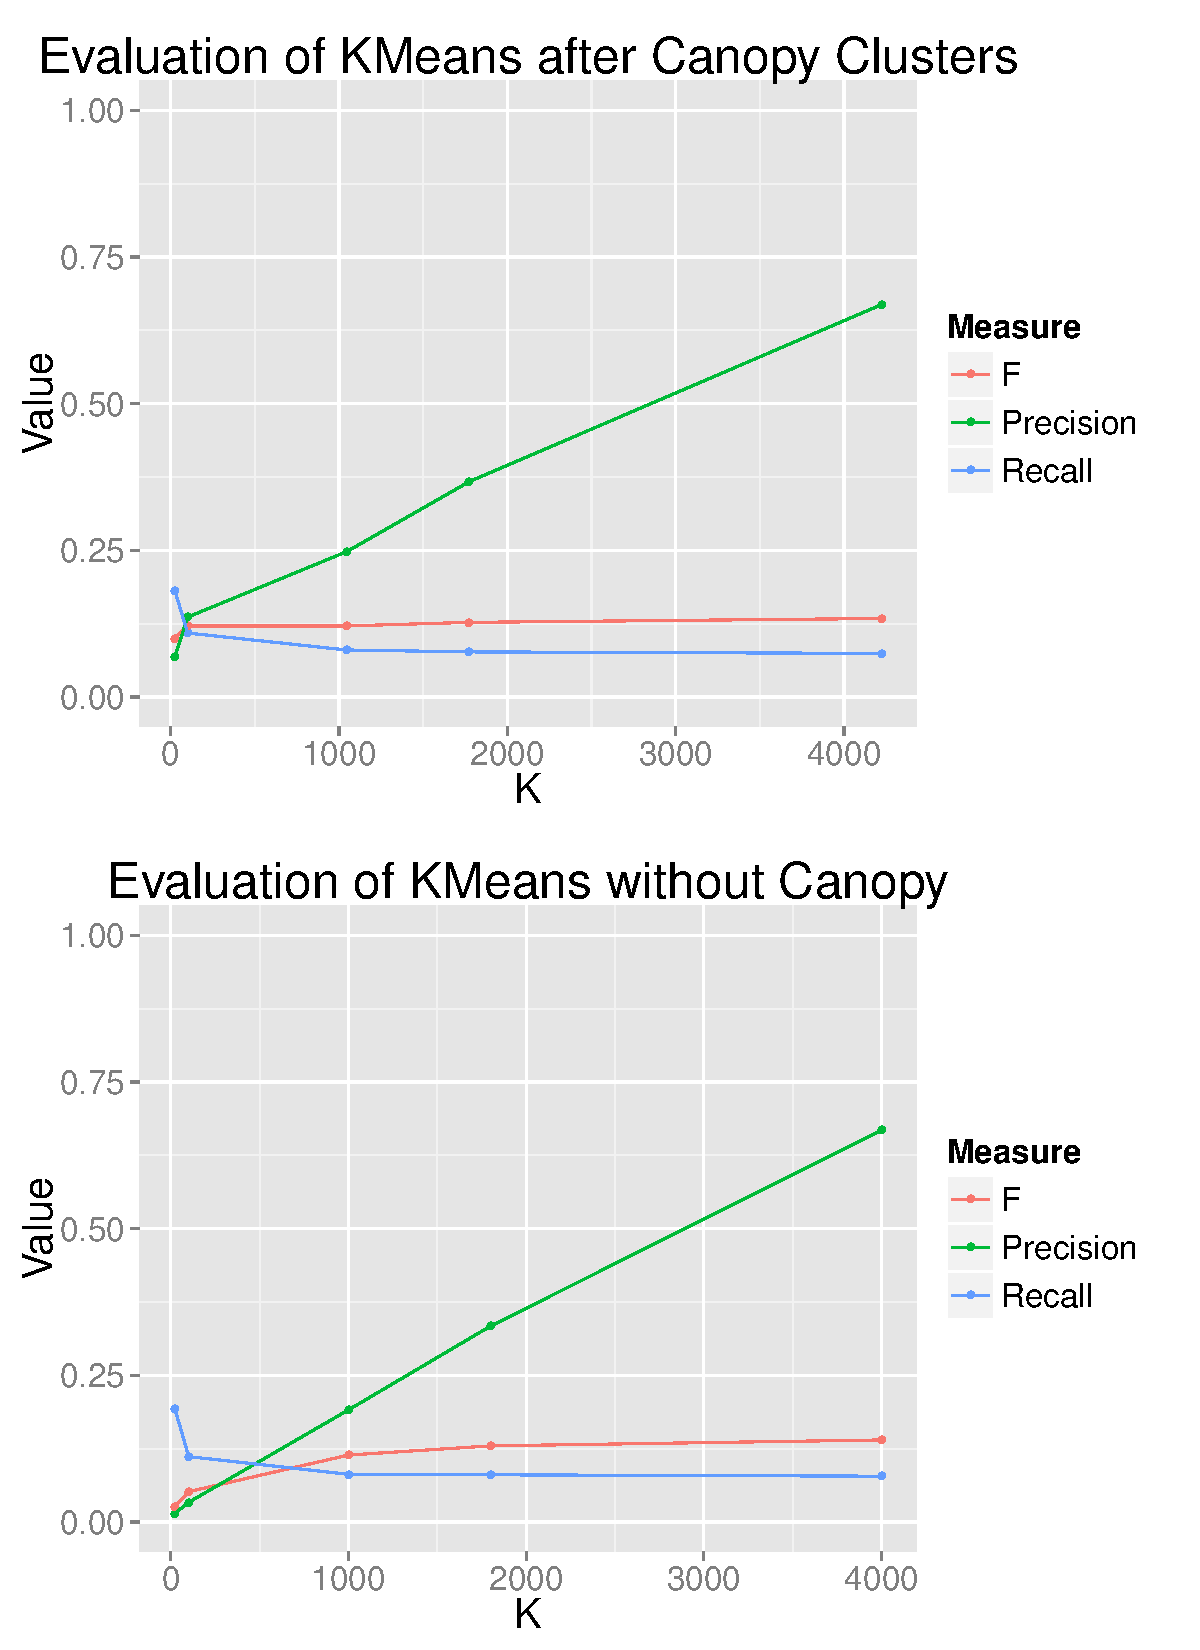
\includegraphics[scale=0.7]{cs689-plots-cluster.pdf}
\end{center}
\caption{The effect of varying $k$ in $k$-means clustering on F score, precision and recall with and without canopies.}
\end{figure}

The next graphs show the difference in precision, recall, and F scores between $k$-means run with the randomized centroids and canopy centroids.

\begin{figure}
\begin{center}
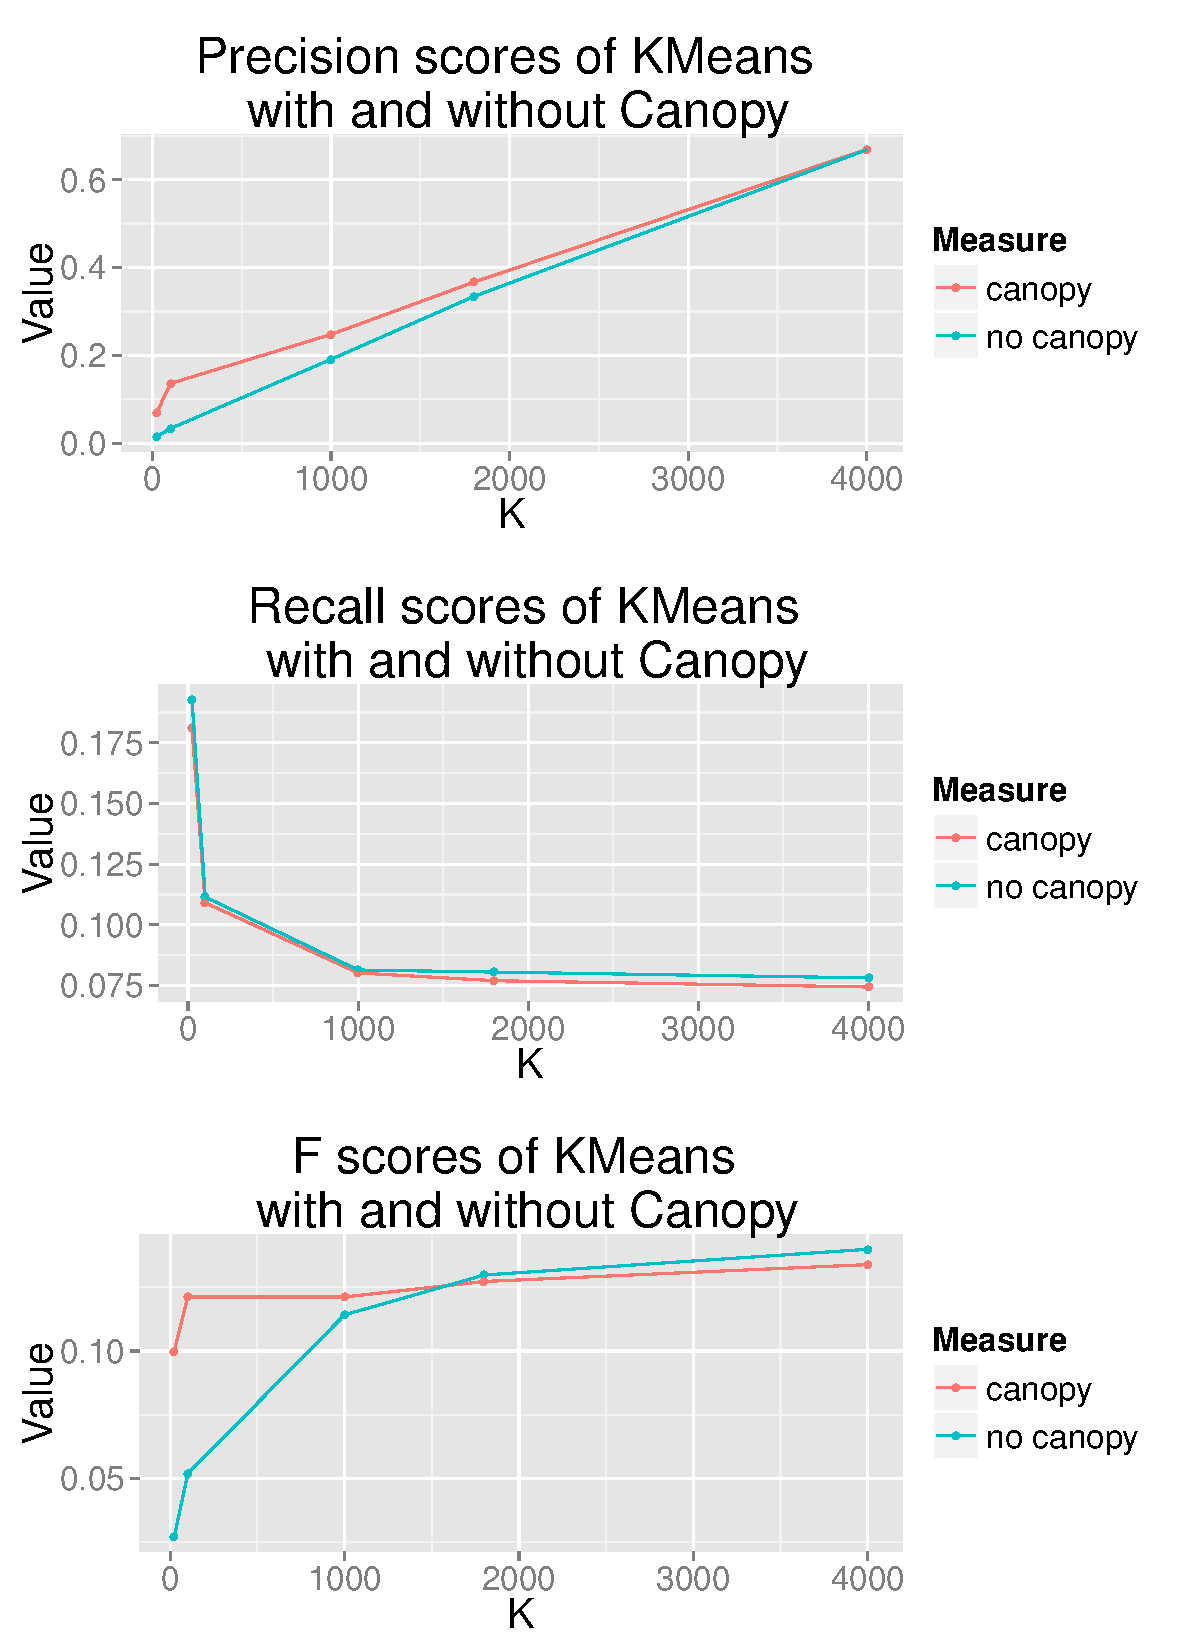
\includegraphics[scale=0.7]{cs689-plots-compare.pdf}
\end{center}
\caption{The effect of bootstrapping using canopies to precision, recall and F score.}
\end{figure}

\subsection{Support Vector Machines}

Multi-class classification using non-linear SVMs is extremely slow on high dimensional data. We therefore were only able to obtain results for linear SVMs. For the experiment with 23 classes, results listed in Figure 5, we split the 7750 examples into 6500 training and 1250 testing examples. The results are averages over 10 trials of splitting the data into 7750/1250 test/train split at random (without replacement).
\begin{figure}
\begin{center}
\begin{tabular}{cc}
\hline
{\bf $C$} & {\bf Error} \\ \hline
1.0 & 91.47 \\
2.0 & 90.83 \\
3.0 & 90.24 \\
4.0 & 89.65 \\
5.0 & 89.94 \\
6.0 & 89.78 \\
7.0 & 90.32 \\
8.0 & 89.94 \\
9.0 & {\bf 89.49} \\
10.0 & 89.50
\end{tabular}
\end{center}
\caption{The effect of varying $C$, the tradeoff between margin size and training error, on classification error by a linear SVM on 23 classes.}
\end{figure}

Clearly, the error rates are high, though above random considering that we are classifying into 23 different classes. Varying $C$, the tradeoff between margin size and training error, made little difference. We also tried varying $C$ in increments of 10 from 10 to 100, which also made little difference.

Seeing these high error rates, we tried running simpler experiments with only 5 classes. In this case we split the data into 1556 training and 300 testing examples, similar relative proportions to the experiment with 23 classes. We did the same averaging over 10 random splits in this case.

\begin{figure}
\begin{center}
\begin{tabular}{cc}
\hline
{\bf $C$} & {\bf Error} \\ \hline
1.0 & 55.50 \\
2.0 & 56.23 \\
3.0 & 54.57 \\
4.0 & 52.73 \\
5.0 & 53.77 \\
6.0 & 53.93 \\
9.0 & 54.53 \\
8.0 & 52.16 \\
7.0 & 52.73 \\
10.0 & {\bf 52.13}
\end{tabular}
\end{center}
\caption{The effect of varying $C$, the tradeoff between margin size and training error, on classification error by a linear SVM on 5 classes.}
\end{figure}

Here we see greatly improved results, hovering around 50\% error, which again is better than random since we are classifying into 5 different classes. There is a stronger trend in this data of results increasing as $C$ increases, but further experimenting with $C$ did not provide significant improvements.

\section{Discussion}
The problem of author identification is a very difficult machine learning problem. Even humans can have a difficult time discerning the authorship of an unknown piece of text. Our initial results leave much room for improvement and future directions of research. The biggest boost in performance would most likely come from further feature engineering, or extracting higher order features from the data such as bigrams, or syntactic dependency pairs. It seems like our features failed to encapsulate the properties of an individual's writing that distinguishes him or her from others. Although we implemented a widely used set of features, there is no definitive set of features for author attribution classification. It is also possible that other classification algorithms may fare better on this task than the support vector machines or clustering algorithms that we tried.

\bibliography{final_report}
\bibliographystyle{unsrt}

%\end{multicols}

\end{document}

%%% Local Variables: 
%%% mode: latex
%%% TeX-master: t
%%% End: 
